In this section we present the results obtained for the SFs in the $\tauhad e$ and $\tauhad \mu$ final states. 
\subsection{Z-$\pt$ Study}
Given that our particular selection of events favours highly boosted $\Zll$ events, the Z$\pt$ is expected to peak at higher values than for normal back to back $\Zll$ events. Previous results \cite{Aad:2019wmn}, have shown that different Monte Carlo generators predict different shapes for the Z$\pt$ distribution, specially in the high-$\pt$ tail. In this analysis, we used two different MC generators for modelling the signal samples, $\POWPY[8]$ (PoPy) and $\SHERPA$. As it can be seen in Fig. \ref{Fig10}, Sherpa does a better job describing the Z boson transverse momentum for high Z$\pt$ values than PoPy. However both generators underestimate the measured value below the Z$\pt=300$ GeV region. 

Then, if we just measure the single ratio defined by equation \ref{eq14}, we would be sensitive to the Z$\pt$ miss-modelling. However, when taking the double ratio this effect should cancel. Additionally, the $Z\to\tauhad\taulep$ and $\Zll$ PoPy samples have been re-weighted according to the data/simulation ratio given in Fig. \ref{Fig10}. We call this samples PoPy-RW. The aim of this procedure is to show that the double ratio method is not sensitive at first order to the Z$\pt$ modelling.

\begin{figure}[htbp]
	\centering
	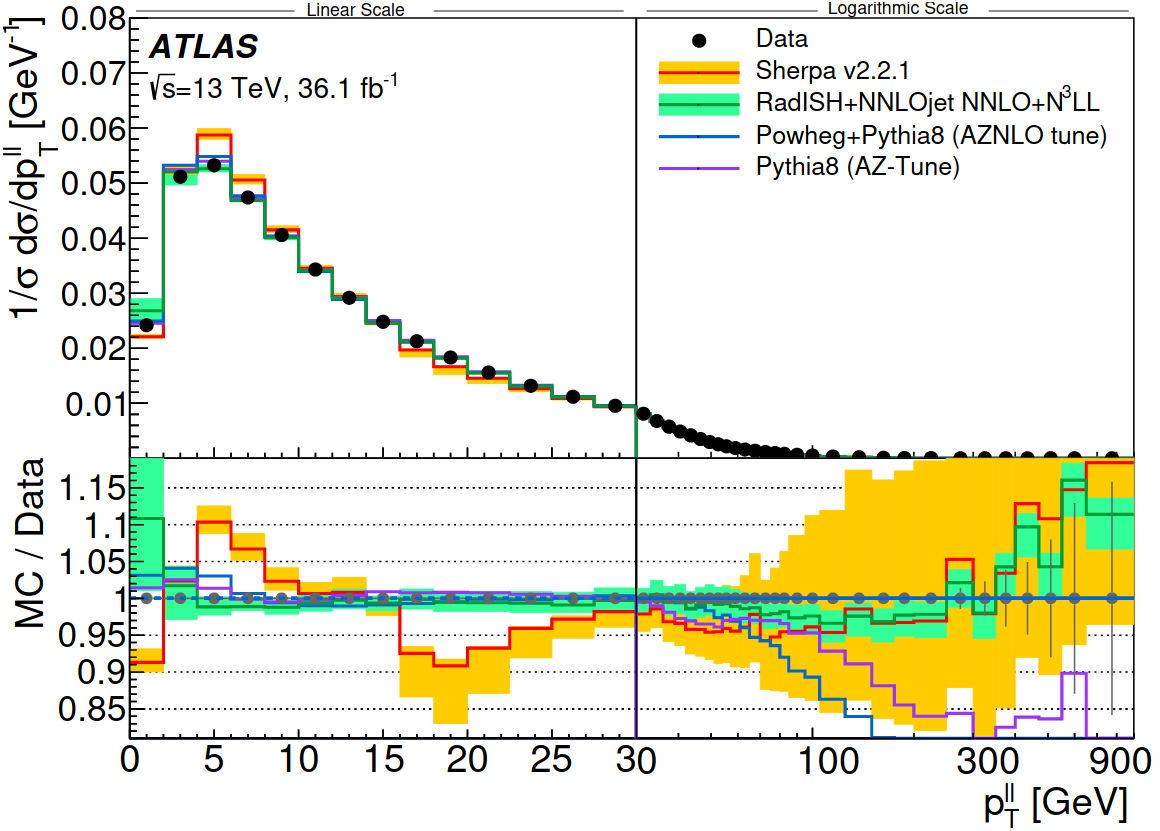
\includegraphics[width=0.6\textwidth]{figures/Fig10}
	\caption{Comparison of the Z$\pt$ modelling in Drell-Yan events made by different MC generators. Taken from \cite{Aad:2019wmn}}
	\label{Fig10}
\end{figure}

Fig. \ref{Fig11}, shows the Z$\pt$ distribution for our final selected events. Looking at these plots, it is clear that $\Sherpa$ does a better job for highly-boosted $\Zll$ events. 

\begin{figure}[htbp]
	\centering
	\subfloat[]{\label{Fig11a}{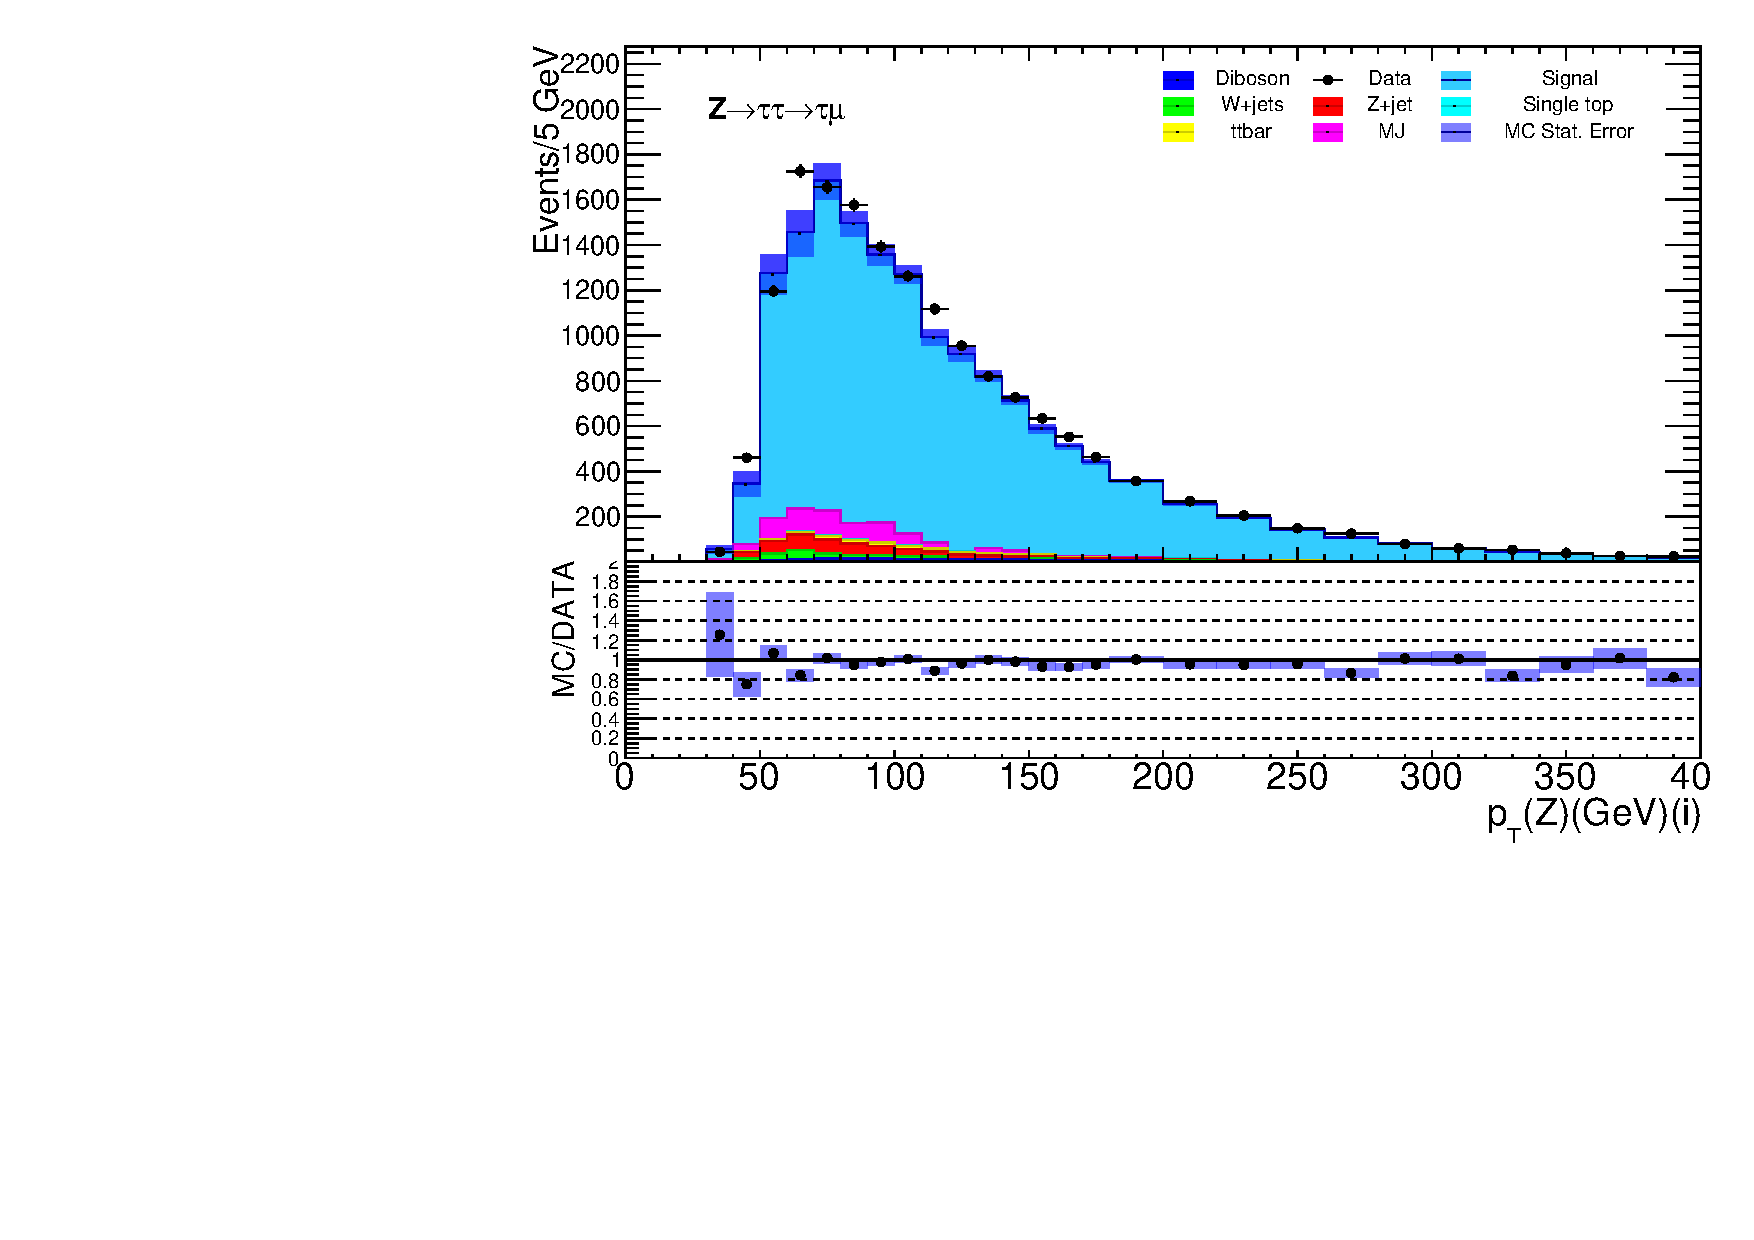
\includegraphics[width=0.50\textwidth]{figures/Fig11a}}}\hfill
	\subfloat[]{\label{Fig11b}{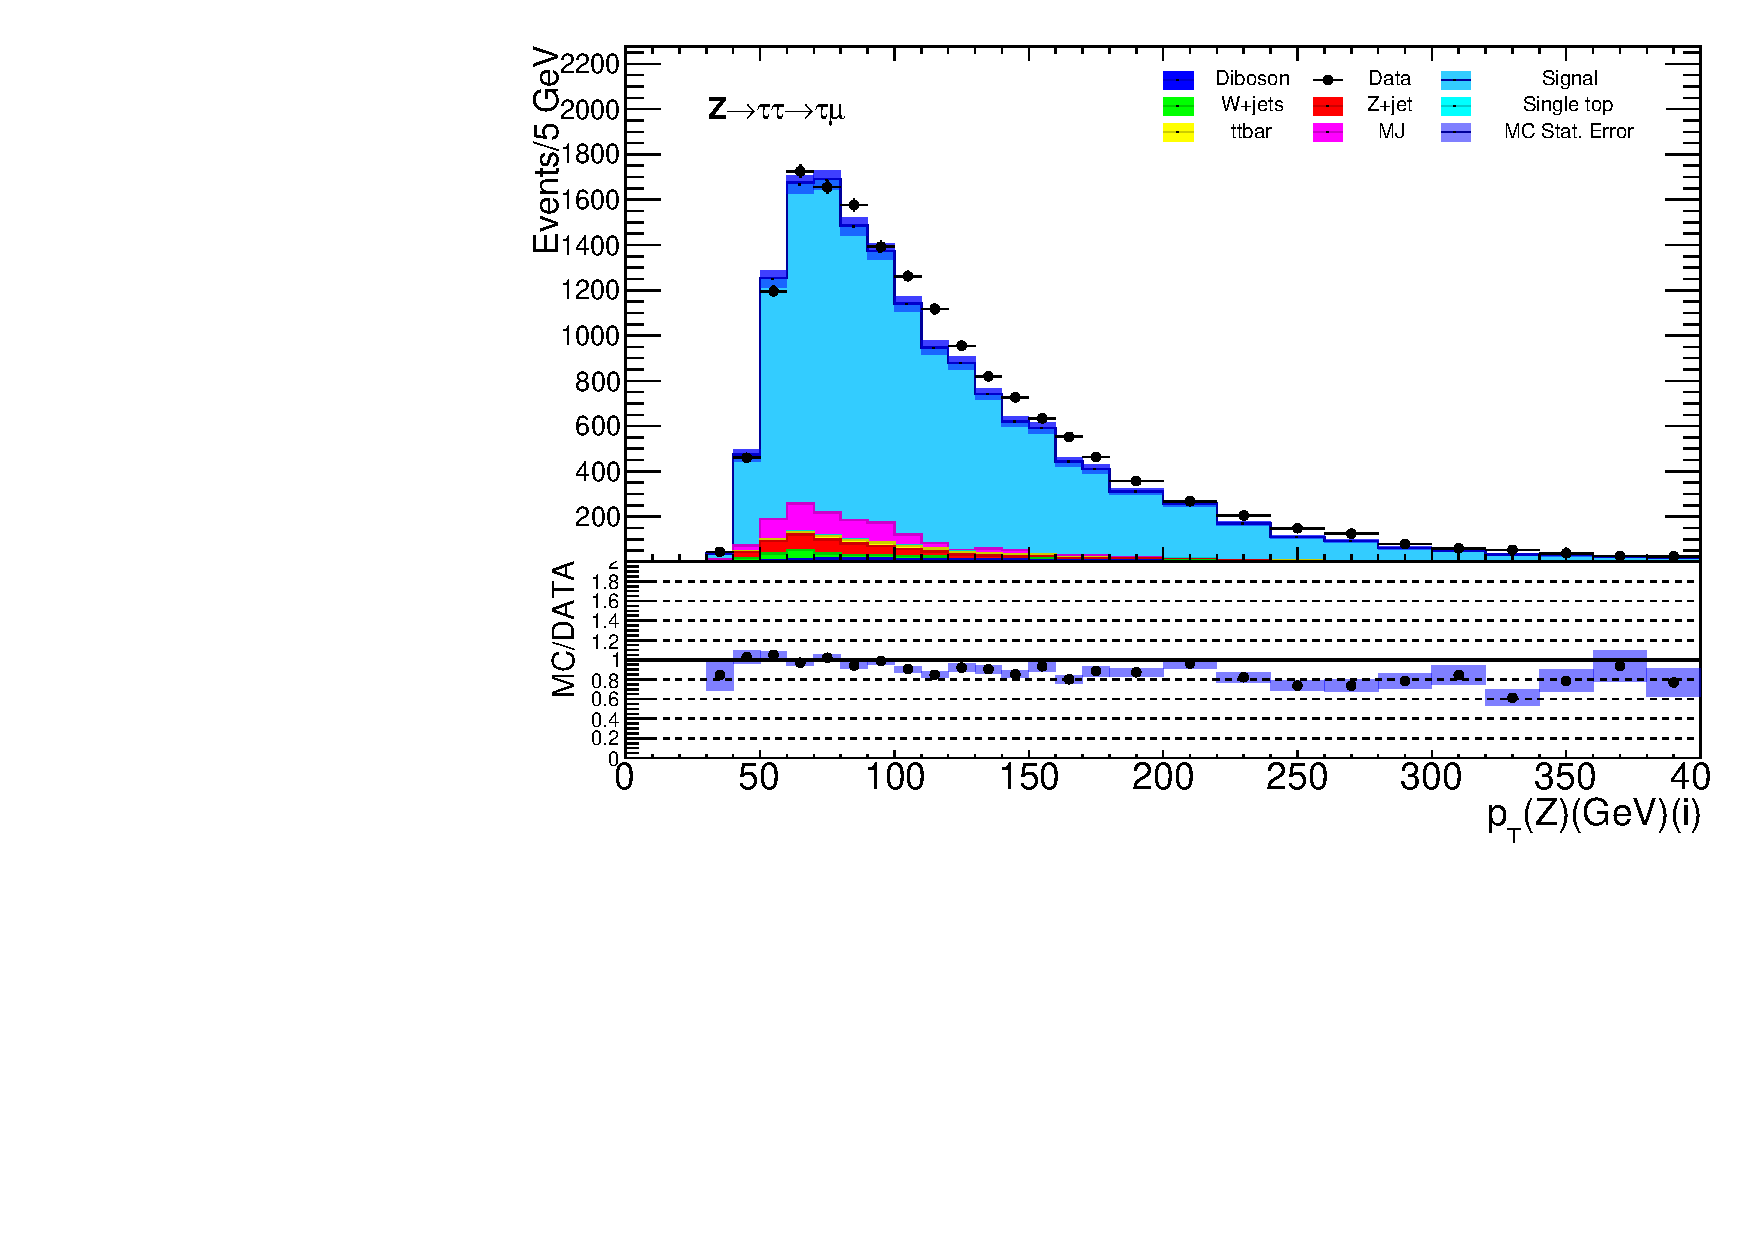
\includegraphics[width=0.50\textwidth]{figures/Fig11b}}}
	\caption{Z$\pt$ distributions for $Z\to\tauhad\mu$ events. $\Sherpa$ prediction (a) is much closer to the data. Meanwhile, $\POWPY[8]$ tends to underestimate the data increasingly as the Z$\pt$ becomes higher. }
	\label{Fig11}
\end{figure}
\subsection{Scale Factors}
The total yields for all the final states, using Sherpa samples as signal, are shown in Table \ref{Tab6}. With these figures, we calculate the C factors and the SFs reported in the second column of Table \ref{Tab7} and \ref{Tab8}. The SFs obtained for the other MC generator configurations are in the two remaining columns.
\begin{table}[]
	\resizebox{\textwidth}{!}{%
		\begin{tabular}{|
				>{\columncolor[HTML]{FFFFFF}}c 
				>{\columncolor[HTML]{FFFFFF}}c 
				>{\columncolor[HTML]{FFFFFF}}c 
				>{\columncolor[HTML]{FFFFFF}}c 
				>{\columncolor[HTML]{FFFFFF}}c 
				>{\columncolor[HTML]{FFFFFF}}c 
				>{\columncolor[HTML]{FFFFFF}}c |}
			\hline
			\multicolumn{1}{|c|}{\cellcolor[HTML]{FFFFFF}\textbf{Final State}}  & \multicolumn{2}{c|}{\cellcolor[HTML]{FFFFFF}\textbf{$Z\to\tauhad\mu$}}                                                              & \multicolumn{1}{c|}{\cellcolor[HTML]{FFFFFF}}                                        & \multicolumn{2}{c|}{\cellcolor[HTML]{FFFFFF}\textbf{$Z\to\tauhad\mu$}}                                                              & \cellcolor[HTML]{FFFFFF}                                     \\ \cline{1-3} \cline{5-6}
			\multicolumn{1}{|c|}{\cellcolor[HTML]{FFFFFF}\textbf{Sample}}       & \multicolumn{1}{c|}{\cellcolor[HTML]{FFFFFF}\textbf{1-Prong}}    & \multicolumn{1}{c|}{\cellcolor[HTML]{FFFFFF}\textbf{3-Prong}}    & \multicolumn{1}{c|}{\multirow{-2}{*}{\cellcolor[HTML]{FFFFFF}\textbf{$Z\to\mu\mu$}}} & \multicolumn{1}{c|}{\cellcolor[HTML]{FFFFFF}\textbf{1-Prong}}    & \multicolumn{1}{c|}{\cellcolor[HTML]{FFFFFF}\textbf{3-Prong}}    & \multirow{-2}{*}{\cellcolor[HTML]{FFFFFF}\textbf{$Z\to ee$}} \\ \hline
			\multicolumn{1}{|c|}{\cellcolor[HTML]{FFFFFF}\textbf{True Signal}}  & \multicolumn{1}{c|}{\cellcolor[HTML]{FFFFFF}$6083.19\pm61.147$}  & \multicolumn{1}{c|}{\cellcolor[HTML]{FFFFFF}$1587.927\pm32.098$} & \multicolumn{1}{c|}{\cellcolor[HTML]{FFFFFF}}                                        & \multicolumn{1}{c|}{\cellcolor[HTML]{FFFFFF}$4656.503\pm58.314$} & \multicolumn{1}{c|}{\cellcolor[HTML]{FFFFFF}$1233.426\pm27.754$} &                                                              \\ \hline
			\multicolumn{1}{|c|}{\cellcolor[HTML]{FFFFFF}\textbf{Fake Signal}}  & \multicolumn{1}{c|}{\cellcolor[HTML]{FFFFFF}$65.163\pm5.726$}    & \multicolumn{1}{c|}{\cellcolor[HTML]{FFFFFF}$1.457\pm1.151$}     & \multicolumn{1}{c|}{\cellcolor[HTML]{FFFFFF}}                                        & \multicolumn{1}{c|}{\cellcolor[HTML]{FFFFFF}$7.337\pm1.598$}     & \multicolumn{1}{c|}{\cellcolor[HTML]{FFFFFF}$0.473\pm0.34$}      &                                                              \\ \hline
			\multicolumn{1}{|c|}{\cellcolor[HTML]{FFFFFF}\textbf{Data}}         & \multicolumn{1}{c|}{\cellcolor[HTML]{FFFFFF}$6731\pm82.043$}     & \multicolumn{1}{c|}{\cellcolor[HTML]{FFFFFF}$1564\pm39.547$}     & \multicolumn{1}{c|}{\cellcolor[HTML]{FFFFFF}$220337\pm469.401$}                      & \multicolumn{1}{c|}{\cellcolor[HTML]{FFFFFF}$5280\pm72.664$}     & \multicolumn{1}{c|}{\cellcolor[HTML]{FFFFFF}$1240\pm35.214$}     & $170783\pm413.259$                                           \\ \hline
			\multicolumn{1}{|c|}{\cellcolor[HTML]{FFFFFF}\textbf{Signal (T+F)}} & \multicolumn{1}{c|}{\cellcolor[HTML]{FFFFFF}$6148.354\pm61.415$} & \multicolumn{1}{c|}{\cellcolor[HTML]{FFFFFF}$1589.384\pm32.118$} & \multicolumn{1}{c|}{\cellcolor[HTML]{FFFFFF}$199195.52\pm361.578$}                   & \multicolumn{1}{c|}{\cellcolor[HTML]{FFFFFF}$4663.841\pm58.336$} & \multicolumn{1}{c|}{\cellcolor[HTML]{FFFFFF}$1233.899\pm27.756$} & $155746.726\pm294.846$                                       \\ \hline
			\multicolumn{1}{|c|}{\cellcolor[HTML]{FFFFFF}\textbf{VV}}           & \multicolumn{1}{c|}{\cellcolor[HTML]{FFFFFF}$141.097\pm2.347$}   & \multicolumn{1}{c|}{\cellcolor[HTML]{FFFFFF}$33.667\pm1.113$}    & \multicolumn{1}{c|}{\cellcolor[HTML]{FFFFFF}$4669.998\pm19.439$}                     & \multicolumn{1}{c|}{\cellcolor[HTML]{FFFFFF}$114.437\pm2.147$}   & \multicolumn{1}{c|}{\cellcolor[HTML]{FFFFFF}$32.386\pm1.12$}     & $3813.414\pm12.897$                                          \\ \hline
			\multicolumn{1}{|c|}{\cellcolor[HTML]{FFFFFF}\textbf{$\Wjets$}}     & \multicolumn{1}{c|}{\cellcolor[HTML]{FFFFFF}$17.595\pm13.611$}   & \multicolumn{1}{c|}{\cellcolor[HTML]{FFFFFF}$0\pm0$}             & \multicolumn{1}{c|}{\cellcolor[HTML]{FFFFFF}$0\pm0$}                                 & \multicolumn{1}{c|}{\cellcolor[HTML]{FFFFFF}$0\pm0$}             & \multicolumn{1}{c|}{\cellcolor[HTML]{FFFFFF}$0\pm0$}             & $8.399\pm8.399$                                              \\ \hline
			\multicolumn{1}{|c|}{\cellcolor[HTML]{FFFFFF}\textbf{$\Zjets$}}     & \multicolumn{1}{c|}{\cellcolor[HTML]{FFFFFF}$65.682\pm4.457$}    & \multicolumn{1}{c|}{\cellcolor[HTML]{FFFFFF}$0.115\pm0.115$}     & \multicolumn{1}{c|}{\cellcolor[HTML]{FFFFFF}$33.153\pm8.899$}                        & \multicolumn{1}{c|}{\cellcolor[HTML]{FFFFFF}$23.516\pm2.641$}    & \multicolumn{1}{c|}{\cellcolor[HTML]{FFFFFF}$0.511\pm0.362$}     & $50.815\pm10.931$                                            \\ \hline
			\multicolumn{1}{|c|}{\cellcolor[HTML]{FFFFFF}\textbf{$\ttbar$}}     & \multicolumn{1}{c|}{\cellcolor[HTML]{FFFFFF}$52.418\pm2.695$}    & \multicolumn{1}{c|}{\cellcolor[HTML]{FFFFFF}$16.07\pm1.472$}     & \multicolumn{1}{c|}{\cellcolor[HTML]{FFFFFF}$169.101\pm4.943$}                       & \multicolumn{1}{c|}{\cellcolor[HTML]{FFFFFF}$43.25\pm2.51$}      & \multicolumn{1}{c|}{\cellcolor[HTML]{FFFFFF}$13.817\pm1.423$}    & $134.426\pm4.393$                                            \\ \hline
			\multicolumn{1}{|c|}{\cellcolor[HTML]{FFFFFF}\textbf{Single top}}   & \multicolumn{1}{c|}{\cellcolor[HTML]{FFFFFF}$8.466\pm0.998$}     & \multicolumn{1}{c|}{\cellcolor[HTML]{FFFFFF}$1.429\pm0.414$}     & \multicolumn{1}{c|}{\cellcolor[HTML]{FFFFFF}$23.166\pm1.741$}                        & \multicolumn{1}{c|}{\cellcolor[HTML]{FFFFFF}$4.56\pm0.753$}      & \multicolumn{1}{c|}{\cellcolor[HTML]{FFFFFF}$2.581\pm0.595$}     & $18.488\pm1.584$                                             \\ \hline
			\multicolumn{1}{|c|}{\cellcolor[HTML]{FFFFFF}\textbf{Multi Jet}}    & \multicolumn{1}{c|}{\cellcolor[HTML]{FFFFFF}$46.577\pm13.825$}   & \multicolumn{1}{c|}{\cellcolor[HTML]{FFFFFF}$10.748\pm13.87$}    & \multicolumn{1}{c|}{\cellcolor[HTML]{FFFFFF}}                                        & \multicolumn{1}{c|}{\cellcolor[HTML]{FFFFFF}$36.887\pm15.695$}   & \multicolumn{1}{c|}{\cellcolor[HTML]{FFFFFF}$0\pm15.695$}        &                                                              \\ \hline
			\multicolumn{1}{|c|}{\cellcolor[HTML]{FFFFFF}\textbf{RQCD}}         & \multicolumn{1}{c|}{\cellcolor[HTML]{FFFFFF}$1.234\pm0.081$}     & \multicolumn{1}{c|}{\cellcolor[HTML]{FFFFFF}$1.723\pm0.178$}     & \multicolumn{1}{c|}{\cellcolor[HTML]{FFFFFF}}                                        & \multicolumn{1}{c|}{\cellcolor[HTML]{FFFFFF}$0.746\pm0.208$}     & \multicolumn{1}{c|}{\cellcolor[HTML]{FFFFFF}$1.26\pm0.342$}      &                                                              \\ \hline
			\multicolumn{7}{|c|}{\cellcolor[HTML]{FFFFFF}\textbf{The uncertainty reported in this table only corresponds to the statistical component.}}                                                                                                                                                                                                                                                                                                                                                          \\ \hline
		\end{tabular}%
		\caption{Yields for all the samples used in the analysis with $\Sherpa$ as signal for $\Zll$ events. The total fakes row is defined by the sum of all EW backgrounds, the MJ contribution and the fakes from the signal sample.}
	\label{Tab6}
}
\end{table}

\begin{table}[]
	\resizebox{\textwidth}{!}{%
		\begin{tabular}{|
				>{\columncolor[HTML]{FFFFFF}}c 
				>{\columncolor[HTML]{FFFFFF}}c 
				>{\columncolor[HTML]{FFFFFF}}c 
				>{\columncolor[HTML]{FFFFFF}}c |}
			\hline
			\multicolumn{1}{|c|}{\cellcolor[HTML]{FFFFFF}\textbf{1-Prong}}                    & \multicolumn{1}{c|}{\cellcolor[HTML]{FFFFFF}\textbf{Sherpa}}               & \multicolumn{1}{c|}{\cellcolor[HTML]{FFFFFF}\textbf{PoPy-RW}}              & \textbf{PoPy}                 \\ \hline
			\multicolumn{4}{|c|}{\cellcolor[HTML]{FFFFFF}Muons}                                                                                                                                                                                                                         \\ \hline
			\multicolumn{1}{|c|}{\cellcolor[HTML]{FFFFFF}$C(Z\to\mu\mu)$}                     & \multicolumn{1}{c|}{\cellcolor[HTML]{FFFFFF}$1.082\pm0.002\pm0.002=0.003$} & \multicolumn{1}{c|}{\cellcolor[HTML]{FFFFFF}$0.994\pm0.002\pm0.001=0.002$} & $1.233\pm0.003\pm0.002=0.003$ \\ \hline
			\multicolumn{1}{|c|}{\cellcolor[HTML]{FFFFFF}$C_{\text{Tight}}(Z\to\tauhad\mu)$}  & \multicolumn{1}{c|}{\cellcolor[HTML]{FFFFFF}$1.041\pm0.014\pm0.011=0.017$} & \multicolumn{1}{c|}{\cellcolor[HTML]{FFFFFF}$1.003\pm0.013\pm0.019=0.023$} & $1.241\pm0.016\pm0.024=0.029$ \\ \hline
			\multicolumn{1}{|c|}{\cellcolor[HTML]{FFFFFF}$SF_{\text{Tight}}(Z\to\tauhad\mu)$} & \multicolumn{1}{c|}{\cellcolor[HTML]{FFFFFF}$0.963\pm0.013\pm0.01=0.016$}  & \multicolumn{1}{c|}{\cellcolor[HTML]{FFFFFF}$1.01\pm0.013\pm0.02=0.024$}   & $1.006\pm0.013\pm0.019=0.024$ \\ \hline
			\multicolumn{4}{|c|}{\cellcolor[HTML]{FFFFFF}Electrons}                                                                                                                                                                                                                     \\ \hline
			\multicolumn{1}{|c|}{\cellcolor[HTML]{FFFFFF}$C(Z\to ee)$}                        & \multicolumn{1}{c|}{\cellcolor[HTML]{FFFFFF}$1.071\pm0.003\pm0.002=0.003$} & \multicolumn{1}{c|}{\cellcolor[HTML]{FFFFFF}$1.026\pm0.003\pm0.001=0.003$} & $1.275\pm0.003\pm0.002=0.004$ \\ \hline
			\multicolumn{1}{|c|}{\cellcolor[HTML]{FFFFFF}$C_{\text{Tight}}(Z\to\tauhad e)$}   & \multicolumn{1}{c|}{\cellcolor[HTML]{FFFFFF}$1.085\pm0.016\pm0.014=0.021$} & \multicolumn{1}{c|}{\cellcolor[HTML]{FFFFFF}$1.043\pm0.015\pm0.023=0.028$} & $1.289\pm0.019\pm0.029=0.034$ \\ \hline
			\multicolumn{1}{|c|}{\cellcolor[HTML]{FFFFFF}$SF_{\text{Tight}}(Z\to\tauhad e)$}  & \multicolumn{1}{c|}{\cellcolor[HTML]{FFFFFF}$1.013\pm0.015\pm0.013=0.02$}  & \multicolumn{1}{c|}{\cellcolor[HTML]{FFFFFF}$1.016\pm0.015\pm0.023=0.027$} & $1.011\pm0.015\pm0.023=0.027$ \\ \hline
			\multicolumn{4}{|c|}{\cellcolor[HTML]{FFFFFF}Statistical uncertainty is reported as Correlated $\pm$ Uncorrelated $=$ Total.}                                                                                                                                               \\ \hline
		\end{tabular}%
	 	\caption{Values obtained for the C-Factors and SFs for different generators configurations, in the case of 1-prong taus. Only the statistical uncertainty is reported. The uncorrelated uncertainties stands for the statistical fluctuations coming from the signal sample and the MJ estimation.}
	\label{Tab7}
	}
\end{table}


 
 \begin{table}[H]
 	\resizebox{\textwidth}{!}{%
 		\begin{tabular}{|cccc|}
 			\hline
 			\multicolumn{1}{|c|}{3-Prong}                             & \multicolumn{1}{c|}{Sherpa}                        & \multicolumn{1}{c|}{PoPy-RW}                       & PoPy                          \\ \hline
 			\multicolumn{4}{|c|}{Muons}                                                                                                                                                                         \\ \hline
 			\multicolumn{1}{|c|}{$C_{\text{Tight}}(Z\to\tauhad\mu)$}  & \multicolumn{1}{c|}{$0.945\pm0.025\pm0.021=0.033$} & \multicolumn{1}{c|}{$0.906\pm0.024\pm0.035=0.042$} & $1.117\pm0.029\pm0.043=0.052$ \\ \hline
 			\multicolumn{1}{|c|}{$SF_{\text{Tight}}(Z\to\tauhad\mu)$} & \multicolumn{1}{c|}{$0.874\pm0.023\pm0.019=0.03$}  & \multicolumn{1}{c|}{$0.911\pm0.024\pm0.036=0.043$} & $0.906\pm0.024\pm0.035=0.042$ \\ \hline
 			\multicolumn{4}{|c|}{Electrons}                                                                                                                                                                     \\ \hline
 			\multicolumn{1}{|c|}{$C_{\text{Tight}}(Z\to\tauhad e)$}   & \multicolumn{1}{c|}{$0.965\pm0.029\pm0.025=0.038$} & \multicolumn{1}{c|}{$0.837\pm0.025\pm0.037=0.044$} & $1.032\pm0.031\pm0.046=0.055$ \\ \hline
 			\multicolumn{1}{|c|}{$SF_{\text{Tight}}(Z\to\tauhad e)$}  & \multicolumn{1}{c|}{$0.901\pm0.027\pm0.024=0.036$} & \multicolumn{1}{c|}{$0.815\pm0.024\pm0.036=0.043$} & $0.81\pm0.024\pm0.036=0.043$  \\ \hline
 			\multicolumn{4}{|c|}{Statistical uncertainty is reported as Correlated $\pm$ Uncorrelated $=$ Total.}                                                                                               \\ \hline
 		\end{tabular}%
 	\caption{Values obtained for the C and SFs for different generators configurations, in the case of 3-prong taus. Only the statistical uncertainty is reported. The uncorrelated uncertainties stands for the statistical fluctuations coming from the signal sample and the MJ estimation.}
 	\label{Tab8}
 	}
 \end{table}
 
The first conclusion we can extract by looking at the last two columns of Table \ref{Tab7} and \ref{Tab7} is that the double ratio method makes this measurement safe from any Z-$\pt$ miss-modelling concern. The fact that C-Factors for PoPy-RW and PoPy samples differ by 25$\%$, but the SFs are consistent between the two MC configurations confirms our hypothesis. When comparing the muon and electron final states for 1-prongs, we see that the PoPy results agree between uncertainties and for Sherpa the agreement is at the 1.7 sigma level. For 3-prongs the situation is reverted, the Sherpa estimate agrees between uncertainties and the PoPy result has a 1.6 sigma deviation.

Given that we do not see big deviations between MC generators, the results for the SFs are combined between the muon and electron final states. In this combination we assume a $\%$100 correlation regarding the systematic uncertainties. The results from the combination are given in Table \ref{Tab9}.
\begin{table}[]
	\resizebox{\textwidth}{!}{%
		\begin{tabular}{|cccc|}
			\hline
			\rowcolor[HTML]{FFFFFF} 
			\multicolumn{4}{|c|}{\cellcolor[HTML]{FFFFFF}\textbf{Combination}}                                                                                                                                                                        \\ \hline
			\rowcolor[HTML]{FFFFFF} 
			\multicolumn{1}{|c|}{\cellcolor[HTML]{FFFFFF}$SF_{\text{Tight}}$} & \multicolumn{1}{c|}{\cellcolor[HTML]{FFFFFF}\textbf{Sherpa}} & \multicolumn{1}{c|}{\cellcolor[HTML]{FFFFFF}\textbf{PoPy-RW}} & \textbf{PoPy}                          \\ \hline
			\rowcolor[HTML]{FFFFFF} 
			\multicolumn{1}{|c|}{\cellcolor[HTML]{FFFFFF}1-Prong}             & \multicolumn{1}{c|}{\cellcolor[HTML]{FFFFFF}$0.983\pm0.038$} & \multicolumn{1}{c|}{\cellcolor[HTML]{FFFFFF}$1.012\pm0.040$}  & \cellcolor[HTML]{FFFFFF}$1.08\pm0.040$ \\ \hline
			\rowcolor[HTML]{FFFFFF} 
			\multicolumn{1}{|c|}{\cellcolor[HTML]{FFFFFF}3-Prong}             & \multicolumn{1}{c|}{\cellcolor[HTML]{FFFFFF}$0.885\pm0.047$} & \multicolumn{1}{c|}{\cellcolor[HTML]{FFFFFF}$0.864\pm0.051$}  & $0.859\pm0.051$                        \\ \hline
		\end{tabular}%
	\caption{Values obtained for the SFs after combining the muon and electron final states. The uncertainty represents both the systematic and statistical components.}
	\label{Tab9}
	}
\end{table} 



